\documentclass[12pt]{beamer}
\usepackage{cmap}
\usepackage[T2A]{fontenc}
\usepackage[utf8]{inputenc}
\usepackage{ifluatex}
\usefonttheme[onlymath]{serif}
\usepackage{svg}
\usepackage{enumerate}
\usepackage{hyperref}
\usepackage{mathtools}
\setbeamertemplate{footline}[frame number]
\definecolor{beamer@darkgreen}{rgb}{0,0.6,0}
\setbeamercolor{normal text}{fg=black,bg=white}
\setbeamercolor{title}{fg=black,bg=beamer@darkgreen}
\setbeamercolor{frametitle}{fg=black,bg=beamer@darkgreen}
\setbeamercolor{background canvas}{parent=normal text}

\usepackage[english,russian]{babel}
\usepackage{graphicx}
\usepackage{listings}
\DeclareMathOperator{\sign}{sign}

\usepackage{enumerate}

\author{Катя Тузова}
\title{Машинное обучение}
\date{}

\subtitle{Лекция 2. Метрические методы классификации}

\begin{document}
\frame{\titlepage}
\begin{frame}[fragile]\frametitle{Разбор ДЗ. Общий алгоритм.}

\begin{lstlisting}[frame=single]
standard_deviation = sys.maxsize
for i in range(len(learnX)):
    polynom = OLS.polyfit(learnX, learnY)
    dev = calc_dev(polynom, learnX, learnY)
    if dev < standard_deviation:
       standard_deviation = sd
    else:
       break
\end{lstlisting}

\end{frame}

\begin{frame}\frametitle{Разбор ДЗ. Вопросы.}
\begin{itemize}
	\item[--] Максимальная степень полинома?
	\item[--] Как использовать test.txt?
\end{itemize}
\end{frame}

\begin{frame}\frametitle{Разбор ДЗ. Число обусловленности.}
${\mu(A) = \Vert A^{-1} \Vert \Vert A \Vert}$\\
\vspace{5mm}
Число обусловленности матрицы показывает насколько матрица близка к вырожденной (для квадратных матриц).\\
\vspace{5mm}
${Ax=b}$  \hspace{15mm}  ${det(A) = 0}$\\
\vspace{5mm}
Если матрица $A$ вырожденная, то для некоторых $b$ решение $x$ не существует, а для других $b$ оно будет неединственным.\\
Если $A$ почти вырожденная, то малые изменения в $A$ и $b$ вызовают очень большие изменения в $x$.

\end{frame}


\begin{frame}\frametitle{Cross-fold validation}
Разобьем исходное множество $X$
на два $L$ и $T$ случайным образом.\\
Будем обучаться на $L$ а проверять результат обучения на $T$.\\
\begin{itemize}
\item[+] Простой и надежный
\item[+] Позволяет оценить распределение на множестве
решений

\end{itemize}
\begin{itemize}
\item[--] Последовательные эксперименты зависимы 
\item[--] Используем мало данных для обучения
\item[--] Непонятно как подбирать соотношения ${\frac{\vert L \vert}{\vert T \vert}}$

\end{itemize}
\end{frame}

\begin{frame}\frametitle{$k$-fold validation}
$X$ разбивается на $k$ частей. Затем на ${k-1}$ частях данных производится обучение модели, а оставшаяся часть данных используется для тестирования.
\end{frame}

\begin{frame}\frametitle{Переобучение на полиномах}

\begin{figure}[htbp]
\centering
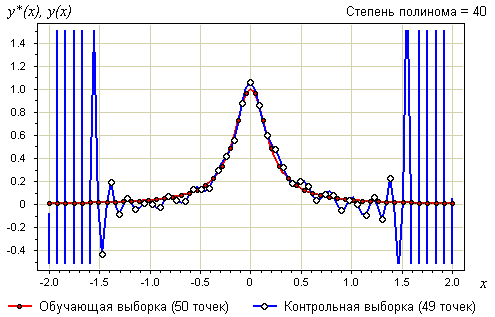
\includegraphics[height=180pt]{overfit}  
\end{figure}

\textcolor{gray}{картинка с machinelearning.ru}

\end{frame}

\begin{frame}\frametitle{Недообучение на полиномах}
\begin{figure}[htbp]
\centering
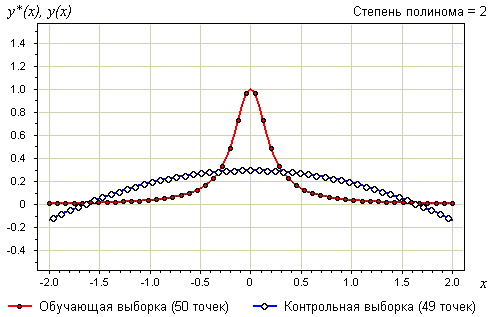
\includegraphics[height=180pt]{underfit}  
\end{figure}

\textcolor{gray}{картинка с machinelearning.ru}
\end{frame}

\begin{frame}\frametitle{Fit на полиномах}
\begin{figure}[htbp]
\centering
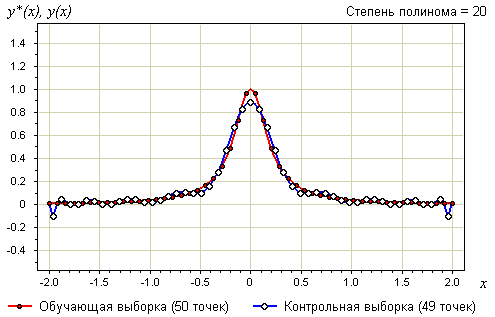
\includegraphics[height=180pt]{fit}  
\end{figure}

\textcolor{gray}{картинка с machinelearning.ru}
\end{frame}
\begin{frame}\frametitle{Как понять какая ситуация. Underfitting}
\begin{figure}[htbp]
\centering
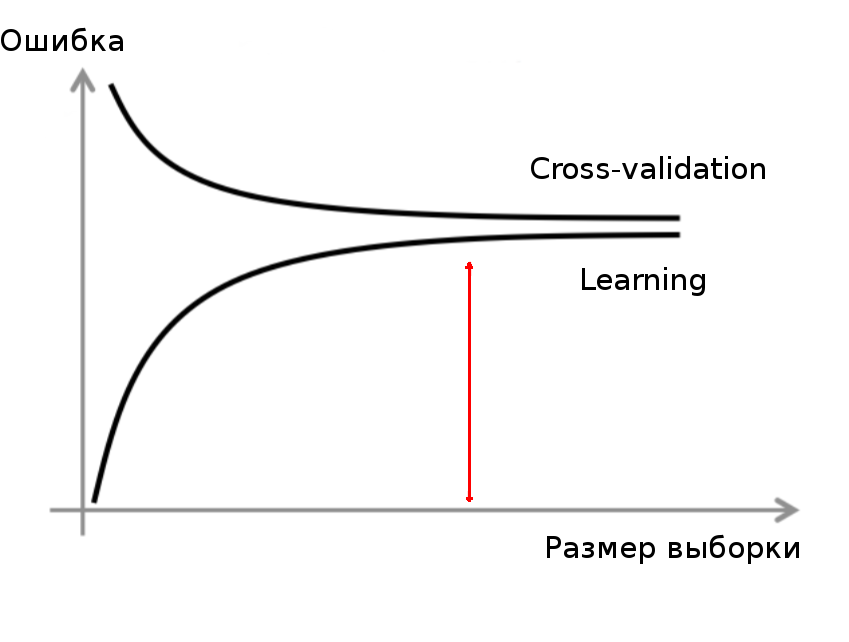
\includegraphics[height=200pt]{underfit1}  
\end{figure}

\end{frame}

\begin{frame}\frametitle{Как понять какая ситуация. Overfitting}
\begin{figure}[htbp]
\centering
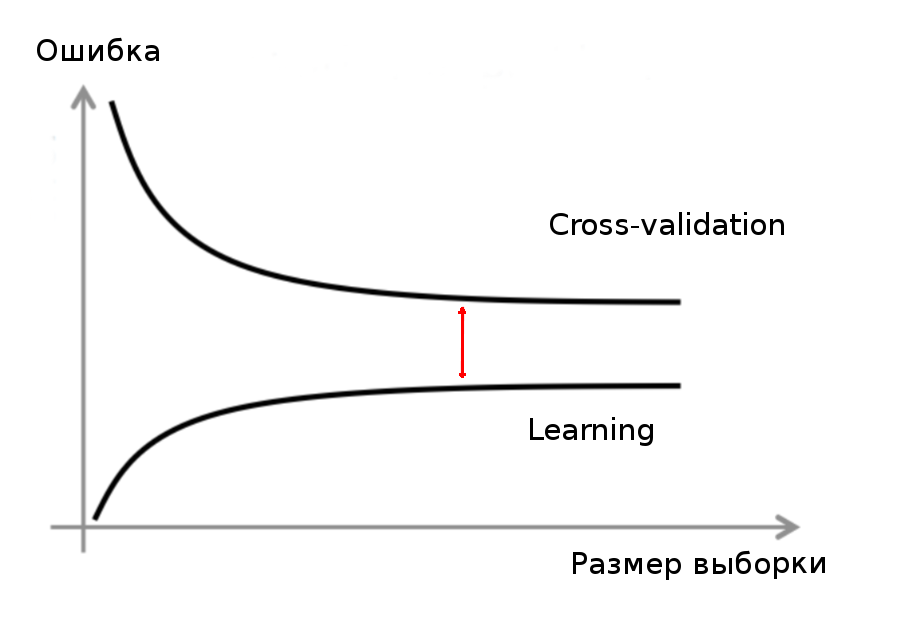
\includegraphics[height=200pt]{overfit1}  
\end{figure}

\end{frame}

\begin{frame}\frametitle{Что в какой ситуации делать}
Переобучение:
\begin{itemize}
\item[--] Увеличение числа объектов для обучения
\item[--] Введение штрафа для определенных степеней полинома
\item[--] Уменьшение количества параметров
\end{itemize}
\vspace{5mm}
Недообучение:
\begin{itemize}
\item[--] Добавление степеней полиному
\item[--] Увеличение количества параметров
\end{itemize}

\end{frame}


\begin{frame}\frametitle{Пример. Ирисы Фишера}
Признаки:\\
\begin{itemize}
	\item[--] длина/ширина чашелистника
	\item[--] длина/ширина лепестка
\end{itemize}
Задача -- разделить на 3 класса
\begin{figure}[htbp]
  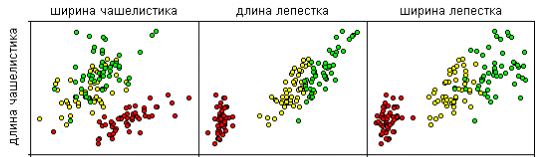
\includegraphics[height=70pt, keepaspectratio = true]{Fisher1}  
\end{figure}
\end{frame}

\begin{frame}\frametitle{Гипотеза компактности}
\textbf{Задача классификации}:\\
$X$ - объекты, $Y$ - ответы (классы)\\
${X^l = (x_i, y_i)_{i=1}^l}$\\
\vspace{5mm}
\textbf{Гипотеза компактности:}\\
Схожие объекты, как правило, лежат в одном классе.\\
\vspace{5mm}
\textbf{"Схожесть":}\\
Функция расстояния = ${\rho: X \times X \rightarrow [0, \infty) }$

\end{frame}

\begin{frame}\frametitle{Примеры функции расстояния}
Евклидово расстояние:\\
${X \in \mathbb{R}^{n}}$\\
\vspace{5mm}
${\rho (u, x_i) = (\sum\limits_{j=1}^n |u^j - x_i^j|^2)^{1/2}}$\\
\vspace{10mm}
%TODO: manhattan, minkovsky (http://www.saedsayad.com/k_nearest_neighbors.htm)
Признаковые описания объектов:\\
${u = \left\{ u^1, u^2, ..., u^n \right\}}$ \\
${x_i = \left\{x_i^1, x_i^2, ..., x_i^n \right\} }$ 
\end{frame}

\begin{frame}\frametitle{Обобщенный метрический классификатор}
$u \in X$ - произвольный объект, который собираемся классифицировать.\\
\vspace{5mm}
Отсортируем объекты $x_1, x_2, ..., x_l$ относительно $u$:
${\rho(u, x_u^1) \leq \rho(u, x_u^2) \leq \dots \leq \rho(u, x_u^l)}$\\
\vspace{5mm}
${x_u^i}$ -- $i$-й сосед объекта $u$\\
${y_u^i}$ -- ответ на $i$-м соседе объекта $u$
 
\end{frame}

\begin{frame}\frametitle{Метрический алгоритм классификации}
${a(u, X^l) = \arg\max\limits_{y \in Y} \underbrace{\sum\limits_{i=1}^l [y_u^i = y]w(i, u)}_{\Gamma_y(u)} }$\\
\vspace{5mm}
$w(i, u)$ - вес $i$-го соседа $u$, неотрицателен\\
$\Gamma_y(u)$ - оценка близости объекта $u$ к классу ${y}$
\end{frame}

\begin{frame}\frametitle{Метод ближайшего соседа}
Объект относится к тому классу, к которому относится ближайший в выборке.\\
${w(i, u) = [i=1]}$\\
\vspace{5mm}
\begin{itemize}
	\item[+] Простота
	\item[+] Интерпретируемость решения
\end{itemize}
\vspace{5mm}
\begin{itemize}
	\item[--	] Неустойчивость к шуму
	\item[--	] Отсутствие настраиваемых параметров
	\item[--	] Низкое качество классификации
	\item[--	] Надо хранить всю выборку целиком		
\end{itemize}
\end{frame}


\begin{frame}\frametitle{Пример.}
\begin{figure}[htbp]
  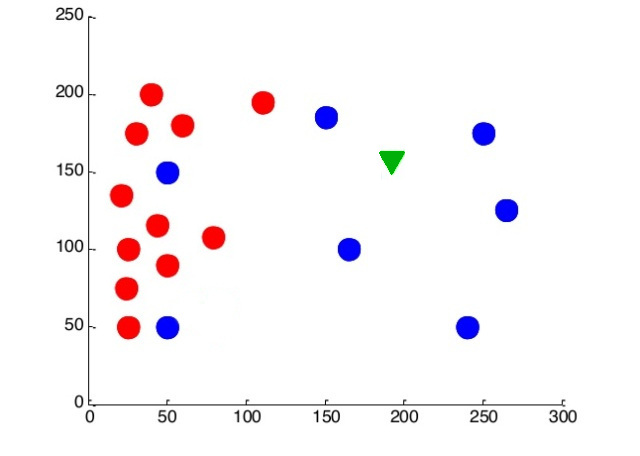
\includegraphics[height=180pt, keepaspectratio = true]{1nearest}  
\end{figure}
\end{frame}

\begin{frame}\frametitle{Пример неустойчивости к шуму}
\begin{figure}[htbp]
  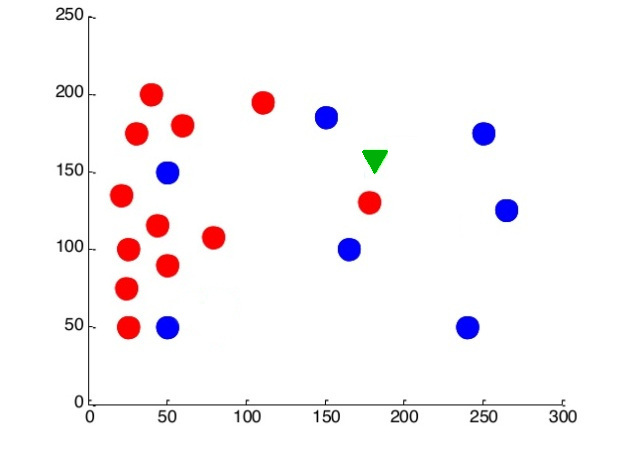
\includegraphics[height=180pt, keepaspectratio = true]{1nearest1}  
\end{figure}
\end{frame}



%\begin{frame}\frametitle{Decision boundaries. Voronoy diagram}
%TODO
%\end{frame}

\begin{frame}\frametitle{Метод k ближайших соседей}
${w(i, u) = [i \leq k]}$\\
\vspace{5mm}
\begin{itemize}
	\item[+] Менее чувствителен к шуму
	\item[+] Появляется настраиваемый параметр k
\end{itemize}
\begin{itemize}
\item[--] Неоднозначность классификации при ${\Gamma_y(u) = \Gamma_s(u), y \neq s}$
\end{itemize}

\end{frame}
\begin{frame}\frametitle{Как выбрать $k$}
Функционал скользящего контроля (leave-one-out):\\
${LOO(k, X^l) = \sum\limits_{i=1}^l [a(x_i; X^l \backslash \left\{x_i\right\}, k) \neq y] \rightarrow \min\limits_k}$\\
\vspace{5mm}

\end{frame}

\begin{frame}\frametitle{Вопрос}
Правда ли надо выбрасывать один объект?
\end{frame}

%\begin{frame}\frametitle{Ответ}
%Картинка
%UCI breast cancer
%смещенное/несмещенное число ошибок
%k = 1 => 0 ошибок, что не правда.\\
%Пример переобучения.
%\end{frame}

\begin{frame}\frametitle{Метод $k$ взвешенных соседей}
${w(i,u) = [i \leq k] * w_i}$, где $w_i$ это вес, зависящий только от номера соседа\\
\vspace{5mm}
Возможные эвристики:\\
\begin{itemize}
\item[--] ${w_i = \frac{k+1-i}{k}}$ -- линейное убывающие веса\\ % почему плохо?
\item[--] ${w_i = q^i}$ -- экспоненциально убывающие веса\\

\end{itemize}
\vspace{5mm}
Проблемa:\\
как более обоснованно задать веса?\\
\end{frame}

\begin{frame}\frametitle{Ядерная оценка плотности}
\textbf{Метод окна Парзена}\\
${w_i = K(\frac{\rho(u, x_u^i)}{h})}$\\
$K(r)$ -- ядро, невозрастающее, положительное на [0, 1]\\
\vspace{8mm} 
Фиксированной ширины:\\
${a(u, X^l, h, K) = \arg\max\limits_{y \in Y} \sum\limits_{i=1}^l [y_u^i = y] K(\frac{\rho(u, x_u^i)}{h})}$\\
$h$ -- ширина окна\\
\vspace{5mm}
Переменной ширины:\\
${a(u, X^l, k, K) = \arg\max\limits_{y \in Y} \sum\limits_{i=1}^l [y_u^i = y] K(\frac{\rho(u, x_u^i)}{\rho(u, x_u^{k+1})})}$

\end{frame}

\begin{frame}\frametitle{Метод окна Парзена}
\begin{figure}[htbp]
  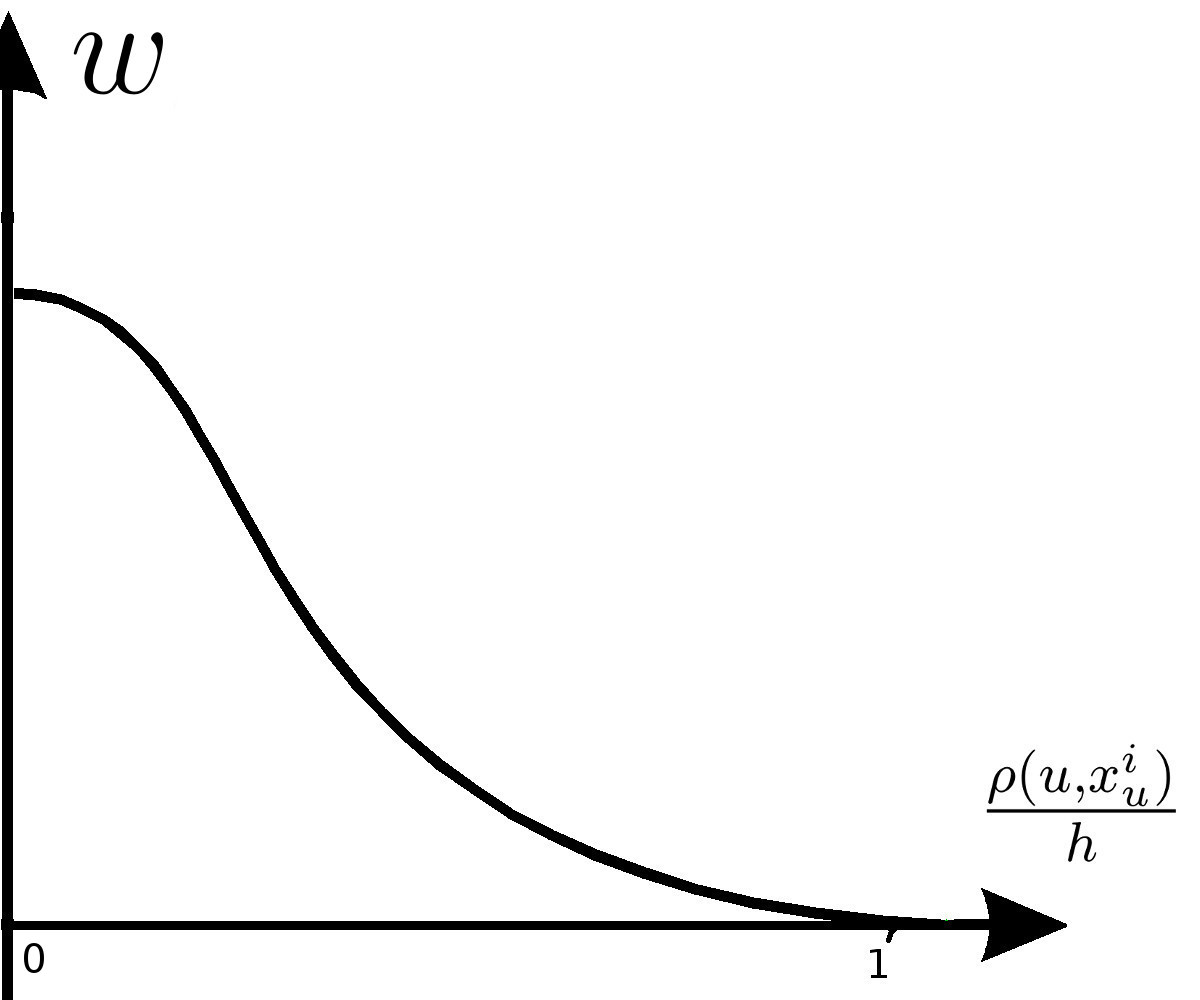
\includegraphics[height=180pt, keepaspectratio = true]{parzen1}  
\end{figure}
\end{frame}

\begin{frame}\frametitle{Выбор метрики}
Какие метрики вам известны?\\
Как выбрать подходящую? 
%http://arxiv.org/pdf/1306.6709v4.pdf
\end{frame}

\begin{frame}\frametitle{Выбор метрики. MMC}
Максимизировать сумму расстояний между объектами разных классов
при этом сохраняя сумму расстояний между объектами одного класса небольшой.\\
\vspace{8mm}
%${\max_{M\in \mathbb{S^d}} \sum_{x_i, x_j \in D} d_M(x_i, x_j) }$\\
${\max \sum\limits_{x_i, x_j \in D} \rho(x_i, x_j) }$\\
\vspace{8mm}
%${\sum_{x_i, x_j \in S} d_M^2(x_i, x_j) \leq 1 }$
${\sum\limits_{x_i, x_j \in S} \rho^2(x_i, x_j) \leq 1 }$
%http://arxiv.org/pdf/1306.6709v4.pdf
\end{frame}

\begin{frame}\frametitle{Проклятие размерности}
Если используемая метрика
${\rho(u, x_u^i)}$
основана на суммировании различий по всем признакам, а число признаков очень велико,
то все точки выборки могут оказаться практически одинаково
далеки друг от друга.\\


\vspace{8mm}
Пример:\\
Набор признаков объекта генерируется подбрасыванием честной монетки $n$ раз. Соответственно
каждый объект описывается вектором $[0, 1]^n$. При таких условиях все объекты будут равноудалены.


%Решение:\\
%Понижении размерности с помощью преобразования пространства признаков, 
%либо путём отбора информативных признаков 
\end{frame}

\begin{frame}\frametitle{Предобработка данных}
Что делать если разные шкалы признаков?
\end{frame}
\begin{frame}\frametitle{Предобработка данных}
Все признаки должны быть представлены "в одном масштабе". \\
В противном случае признак с наибольшими числовыми значениями будет доминировать в метрике
\end{frame}


\begin{frame}\frametitle{Жадное добавление признаков}
\begin{itemize}
\item[--] ${\rho_j(u, x_i) = \vert u^j - x_i^j \vert}$ -- расстояние по j-му признаку\\
$LOO(j) \rightarrow \min$\\
\item[--] Добавляем признак и строим $\rho'$\\
${\rho'(u, x_i) = \rho(u, x_i) + w_j\rho_j(u, x_i)}$\\
$LOO(j, w_j) \rightarrow \min$\\
\item[--] Замена признака:\\
${\rho'(u, x_i) = \rho(u, x_i) - w_k\rho_k(u, x_i) + w_j\rho_j(u, x_i)}$\\
\item[--] Добавляем признаки, пока LOO не увеличивается
\end{itemize}

\end{frame}
\begin{frame}\frametitle{Сверхбольшие выборки}
\begin{itemize}
\item[--] Проблема хранения
\item[--] Проблема быстрого поиска ближайших соседей
\end{itemize}
\end{frame}

\begin{frame}\frametitle{Отступ}
Отступ показывает степень "типичности объекта".\\
\vspace{5mm}
Отступом объекта ${x_i \in X^l}$ относительно классификатора $a$ называется величина\\
${M(x_i) = \Gamma_{y_i}(x_i) - \max\limits_{y \in Y\backslash y_i} \Gamma_y(x_i)}$

\end{frame}

\begin{frame}\frametitle{Типы объектов}
\begin{itemize}
	\item[--] Эталонные
	\item[--] Неинформативные
	\item[--] Пограничные	
	\item[--] Ошибочные	
	\item[--] Шумовые	
\end{itemize}
\end{frame}

\begin{frame}\frametitle{Типы объектов}

\begin{figure}[htbp]
\centering
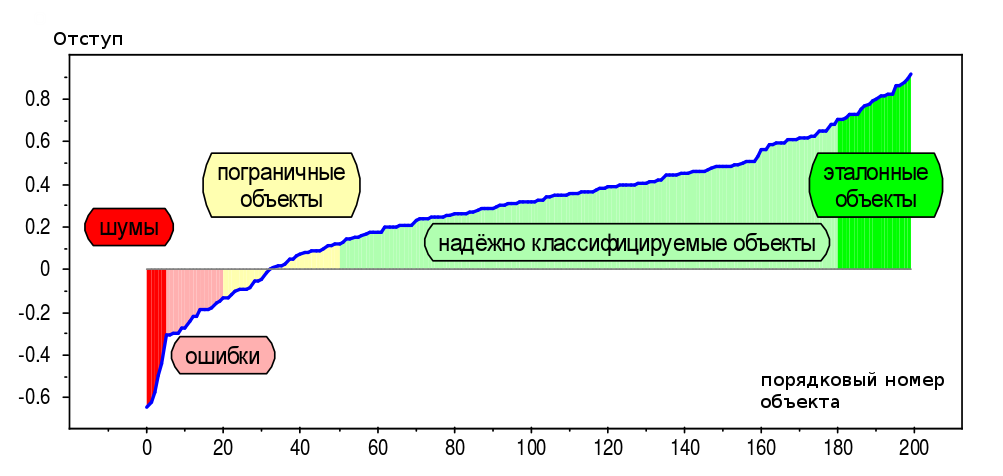
\includegraphics[height=150pt]{margin}  
\end{figure}

\textcolor{gray}{картинка с machinelearning.ru}
\end{frame}

\begin{frame}\frametitle{Отбор эталонных объектов}
Задача:\\
выбрать оптимальное подмножество эталонов $\Omega\subseteq X^l$\\ 
\vspace{5mm}
Классификатор будет иметь вид:\\
${a(u, \Omega) = \arg\max\limits_{y \in Y} \sum\limits_{x_i \in \Omega} [y_u^i = y]w(i, u) }$\\
\end{frame}

\begin{frame}\frametitle{Алгоритм STOLP}
\begin{itemize}
\item[--] Исключить выбросы и пограничные объекты
\item[--] Найти по одному эталону в каждом классе
\item[--] Добавлять эталоны, пока есть отрицательные отступы
\end{itemize}
\end{frame}

\begin{frame}\frametitle{Алгоритм STOLP}

\begin{itemize}
\item[+] Сокращается число хранимых объектов
\item[+] Сокращается время классификации
\item[+] Объекты разделяются по величине отступа
\end{itemize}
\vspace{5mm}
\begin{itemize}
\item[--] Выбор параметра для определения выбросов
\item[--] Не высокая эффективность
\end{itemize}
\end{frame}

%\begin{frame}\frametitle{Полный скользящий контроль}
%Complete cross-validation:\\
%${CCV(X^L) = \frac{1}{C_L^l}\sum }\frac{1}{k}\sum_{x_i \in X^k} [a(x_i, X^l) \neq y_i]$\\
%При k = 1 ${CCV \eq LOO}$
%\end{frame}

\begin{frame}\frametitle{Как быстро искать ближайших соседей}
\begin{itemize}
\item[--] граф ближайших соседей
\item[--] k-d дерево
\item[--] хеширование (LSH)
\end{itemize}

\end{frame}


%\begin{frame}\frametitle{k-d дерево}

%\begin{figure}[htbp]
%\centering
%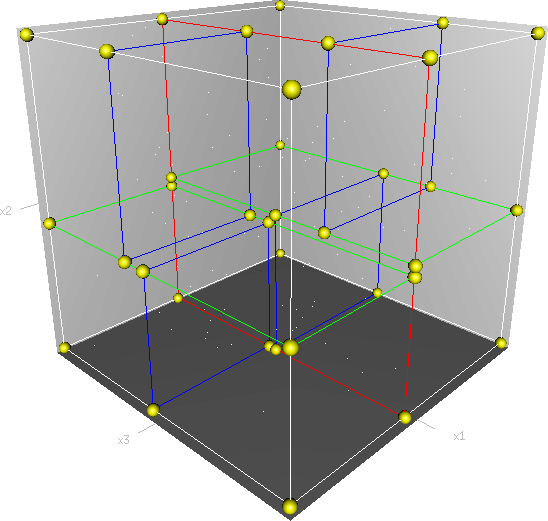
\includegraphics[height=200pt]{3dtree}  
%\end{figure}

%\end{frame}

%\begin{frame}\frametitle{Жадный алгоритм}
%\end{frame}

%\begin{frame}\frametitle{Полный скользящий контроль CCV}
%\end{frame}

%\begin{frame}\frametitle{Профиль компактности}
%\end{frame}

%\begin{frame}\frametitle{Что происходит сейчас в области knn}
%A Ranking-based KNN Approach for Multi-Label Classification 2012
% http://jmlr.org/proceedings/papers/v25/chiang12/chiang12.pdf

%Fast Approximate kNN Graph Construction for High Dimensional
%Data via Recursive Lanczos Bisection 2009
%http://www.jmlr.org/papers/volume10/chen09b/chen09b.pdf

%mahalanobis Distance Metric Learning for Large Margin
%Nearest Neighbor Classification 2009
%http://www.jmlr.org/papers/volume10/weinberger09a/weinberger09a.pdf
%\end{frame}


\begin{frame}\frametitle{Доп. ресурсы}

\href{http://www.machinelearning.ru}{http://www.machinelearning.ru}\\
\vspace{8mm}
\href{http://www.machinelearning.ru/wiki/images/6/6d/Voron-ML-1.pdf}{Пособие}

\end{frame}

\begin{frame}\frametitle{Вопросы по курсовым проектам}

\end{frame}

\begin{frame}\frametitle{На следующей лекции}
\begin{itemize}
\item[--] Кластеризация.  K-means.
\item[--] Цели кластеризации.
\item[--] Типы кластерных структур.
\item[--] Функционал качества кластеризации
\item[--] К-средних
\item[--] Иерархическая кластеризация.
\end{itemize}
\end{frame}
\end{document}
